\begin{figure}[H]
	\centering
	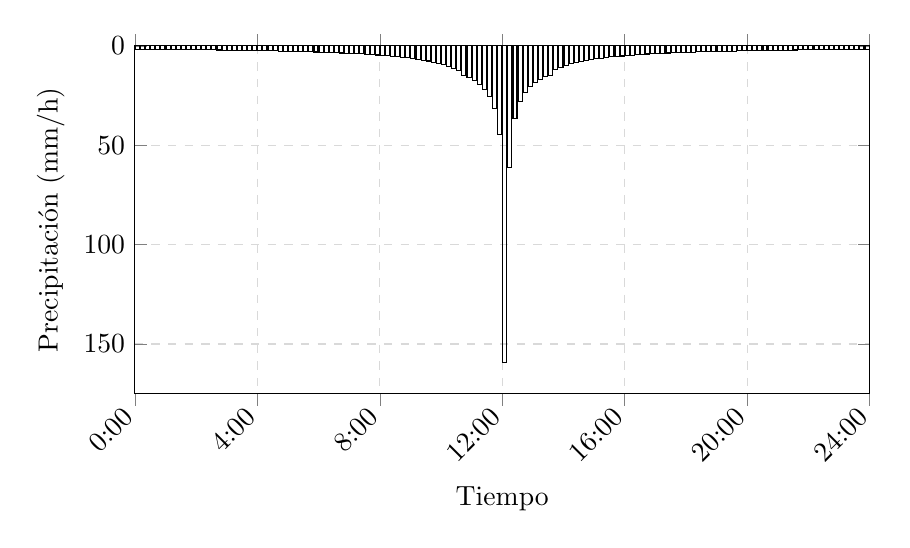
\begin{tikzpicture}
		\begin{axis}[
			width=0.9\textwidth,
			height=6cm,
			xlabel={Tiempo},
			ylabel={Precipitación (mm/h)},
			y dir=reverse,
			ymin=0,
			ymax=175,
			xmin=0,
			xmax=1440,
			ybar,
			bar width=8,
			xtick={0, 240, 480, 720, 960, 1200, 1440},
			xticklabels={0:00, 4:00, 8:00, 12:00, 16:00, 20:00, 24:00},
			xticklabel style={rotate=45, anchor=east},
			grid=major,
			grid style={dashed, gray!30},
			]
			\addplot [
			draw=black,
			fill=none
			]
			coordinates {
				(5, 1.68) (15, 1.68) (25, 1.74) (35, 1.74) (45, 1.74)
				(55, 1.80) (65, 1.80) (75, 1.86) (85, 1.86) (95, 1.86)
				(105, 1.92) (115, 1.98) (125, 1.98) (135, 1.98) (145, 2.04)
				(155, 2.04) (165, 2.10) (175, 2.16) (185, 2.16) (195, 2.22)
				(205, 2.28) (215, 2.28) (225, 2.34) (235, 2.40) (245, 2.46)
				(255, 2.46) (265, 2.52) (275, 2.58) (285, 2.64) (295, 2.70)
				(305, 2.76) (315, 2.82) (325, 2.88) (335, 2.94) (345, 3.06)
				(355, 3.12) (365, 3.18) (375, 3.30) (385, 3.36) (395, 3.48)
				(405, 3.60) (415, 3.72) (425, 3.84) (435, 3.90) (445, 4.08)
				(455, 4.26) (465, 4.44) (475, 4.62) (485, 4.74) (495, 4.98)
				(505, 5.22) (515, 5.46) (525, 5.70) (535, 6.06) (545, 6.36)
				(555, 6.72) (565, 7.20) (575, 7.62) (585, 8.22) (595, 8.82)
				(605, 9.54) (615, 10.38) (625, 11.40) (635, 12.60) (645, 15.00)
				(655, 16.14) (665, 17.58) (675, 19.38) (685, 21.90) (695, 25.56)
				(705, 31.62) (715, 44.58) (725, 159.42) (735, 61.02) (745, 36.54)
				(755, 28.08) (765, 23.52) (775, 20.58) (785, 18.48) (795, 16.80)
				(805, 15.60) (815, 14.94) (825, 12.00) (835, 10.86) (845, 9.96)
				(855, 9.12) (865, 8.46) (875, 7.86) (885, 7.38) (895, 6.90)
				(905, 6.54) (915, 6.18) (925, 5.88) (935, 5.58) (945, 5.28)
				(955, 5.10) (965, 4.86) (975, 4.68) (985, 4.44) (995, 4.32)
				(1005, 4.14) (1015, 4.08) (1025, 3.90) (1035, 3.78) (1045, 3.60)
				(1055, 3.54) (1065, 3.48) (1075, 3.36) (1085, 3.24) (1095, 3.18)
				(1105, 3.06) (1115, 3.00) (1125, 2.94) (1135, 2.88) (1145, 2.82)
				(1155, 2.70) (1165, 2.70) (1175, 2.64) (1185, 2.58) (1195, 2.52)
				(1205, 2.46) (1215, 2.40) (1225, 2.34) (1235, 2.34) (1245, 2.28)
				(1255, 2.22) (1265, 2.16) (1275, 2.16) (1285, 2.16) (1295, 2.10)
				(1305, 2.04) (1315, 2.04) (1325, 1.98) (1335, 1.98) (1345, 1.92)
				(1355, 1.92) (1365, 1.86) (1375, 1.86) (1385, 1.80) (1395, 1.80)
				(1405, 1.74) (1415, 1.74) (1425, 1.74) (1435, 1.68)
			};
		\end{axis}
	\end{tikzpicture}
	\caption{Hietograma - BLOCKS24 $T_r$=25 años (P=178.7 mm)}
	\label{fig:hyeto_desbordes_blocks24_Tr25}
\end{figure}
